\chapter*{Introduction}
\section*{Statistical Learning}
Assume we observed a quantitative response $Y$ and $p$ different predictors $X_1,\dots,X_p$. We assume that there is some relationship between $Y$ and $X=(X_1,\dots,X_p)$, which can be written in the form
$$
Y_i=f(X_i)+\epsilon_i
$$
where $f$ is a fixed but unknown function and $\epsilon_i$ is a random error term, which is independent of $X$ and has mean zero.  

The aim of statistical learning is to estimate the relationship between the predictors and the response (also called dependent variable) starting from the data.

Vorremmo capire la relazione tra le variabili indipendenti e la variabile dipendente basandoci sui dati.
\section*{Data Analysis}
Data Analysis is the process of extracting information from data. Although data and information are often used interchangeably, they are not the same. Data is something that should cointain information, but it is not information itself. In order to extract information from data, we need to build a learning system.

An important thing to know is that when the learning system is \textit{good}, then by increasing the amount of data we have, the available information cannot decrease. In practice, most of the times we do not have a good system (due to analytical, computational, or time skills not available), so it can happen that the data fed to the system is misleading and the information we get from the analysis decreases. A \textit{non optimal} system could be attacked using fake data in order to decrase information and make the system less reliable; the \textit{optimal} system is able to discard that data.

The two main families of problems in data analysis are \textit{estimation} and \textit{classification}. The main difference is that in the estimation problem,
we have a set of data and we want to estimate a real value, while in the classification problem the output is contained in a finite set. This difference is projected onto the output response variable $Y$.

\begin{figure}
    \centering
    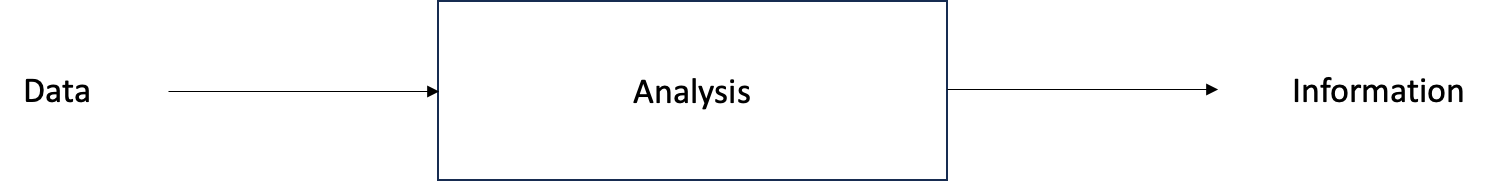
\includegraphics[width=0.7\textwidth]{./figures/chapter_2/data2information.png}
    \caption{The general process of extracting information from data.}
    \label{fig:data2information}
\end{figure}

The input of the learning system can be anything (a vector, a matrix, a graph, a sequence, etc.), but the output is always a real number or a finite set of values. In general,
we do not care about the dimension of the output, because we can always repeat the problem as many times as the dimension of the output.

% qualcosa sul fatto che esiste model based analysis e supervised parametric e non parametric

Data analysis problems don't necessary require a \textit{training phase}. We can have two scenarios:
\begin{enumerate}
    \item \textbf{Model-Based}, the model is given to us.

          \begin{figure}
              \centering
              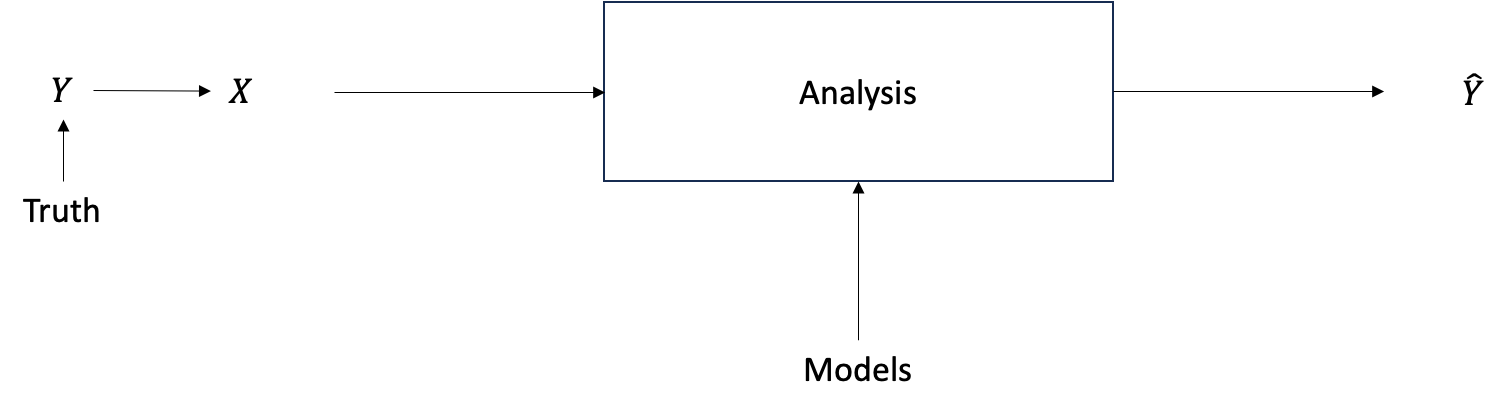
\includegraphics[width=0.7\textwidth]{./figures/chapter_2/modelbased.png}
              \caption{The model based process of extracting information from data.}
              \label{fig:modelbased}
          \end{figure}

          Figure \ref{fig:modelbased} show the scenario. The truth $Y$ influences the data $X$, hidden in it.

          \callout{Note}{Another thing to make clear is that in statistical learning, we do not have a temporal correlation between the variables. When we say that two variables depend on each other, we just mean that they are correlated, without implying the causality.}

    \item \textbf{Model Learning}, we have to learn a statistical characterization of the couple $(X,Y)$.

          \begin{figure}
              \centering
              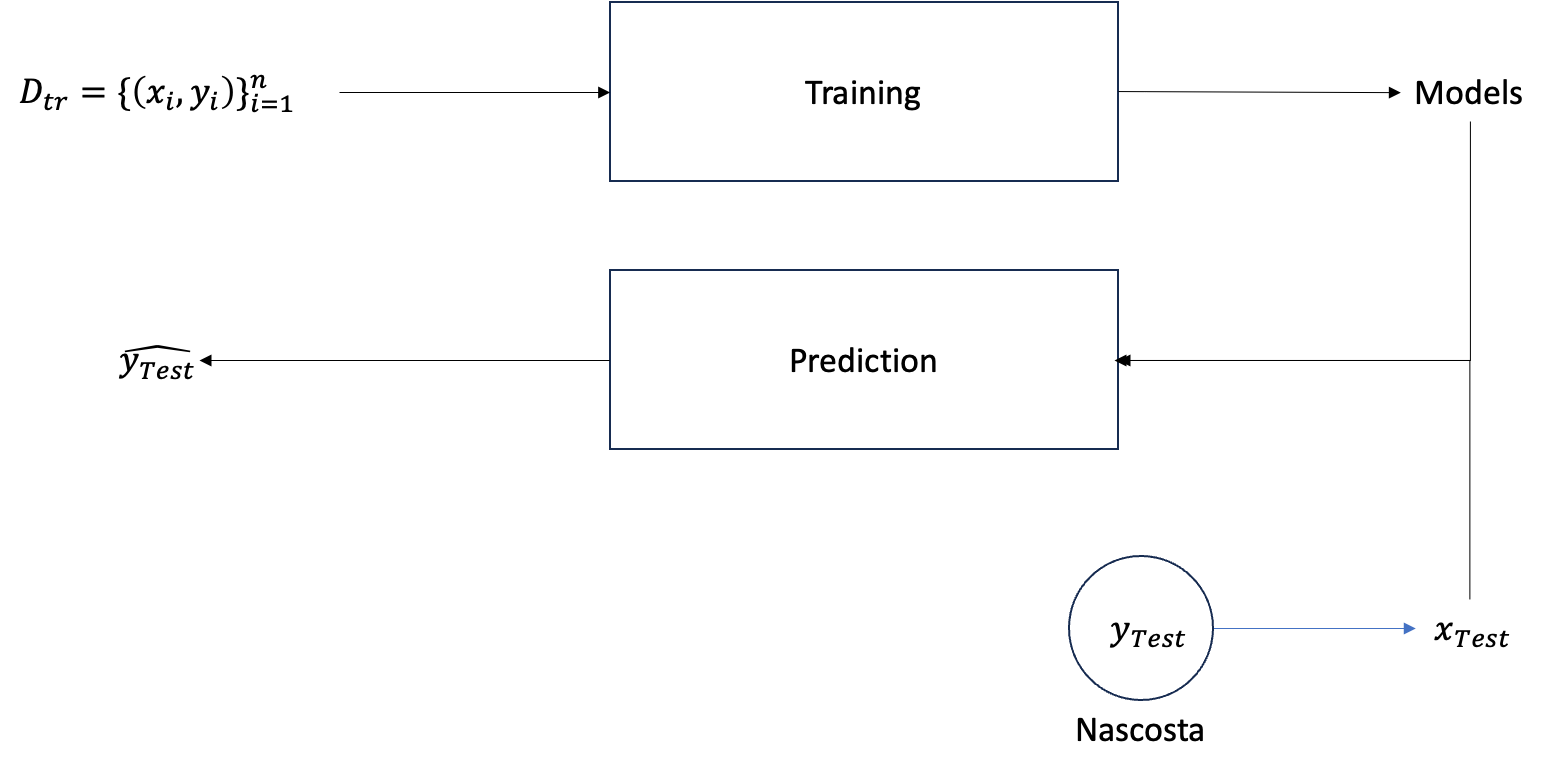
\includegraphics[width=0.7\textwidth]{./figures/chapter_2/modellearning.png}
              \caption{The model learning process of extracting information from data.}
              \label{fig:modellearning}
          \end{figure}

          This scenario could be seen as a \textit{supervised learning} problem when we starts from a set of examples $\mathcal{D}$ to learn the model.
          \[
              \mathcal{D} = \left\{ x_i, y_i \right\}_{i=1}^{N}
          \]
          Figure \ref{fig:modellearning} explain this scenario.


\end{enumerate}
